\chapter{Analysis of the results}
\section{Physical setting}
here explain all the physical concerns of the system, like start from describing the system as 2 quantum systems psir and psil, then write the hamiltonian and describe what are the matrix elements. explain in detail the t element (offdiagonal term) and then introduce the theory of WKB and how it can be used to recover that term. then see from the matrix that the splitting is proportional to t and from WKB that t is proportional to the exponenital of the V applied --> so the splitting is proportional to the exponential o the V applied. Then show the results (next section) and after see the fit and comment on how the fit is close to the expiremntal results.
\section{Energy splittings and fitting of the results}
In our simulation, the energy splittings between the ground states of the two dots are reported in the following table:
\begin{table}[H]
    \centering
    \begin{tabular}{|l|c|}
        \hline
        \textbf{Barrier Voltage (V)} & \textbf{Energy splitting ($\mu$eV )}\\ \hline
        3.69 & 2.08 \\ \hline
        3.80 & 2.91 \\ \hline
        3.90 & 3.83 \\ \hline
        3.99 & 4.84 \\ \hline
        4.09 & 5.94 \\ \hline
        4.19 & 7.20 \\ \hline
    \end{tabular}
\end{table}
We then fitted the experimental data to an exponential function of the form:
\begin{equation}
    y = a \cdot e^{b \cdot x}
\end{equation}
where $y$ in this case represents the energy splitting and $x$ is the barrier voltage. The showed function has been optimized to best fit the experimental data and the parameters $a$ and $b$ have been determined, resulting in $5.11e-10$ and $22.79$ respectively.\\
The plot of the fitted curve and the experimental data is shown in figure \ref{plot}:
\begin{figure}[H]
    \centering
    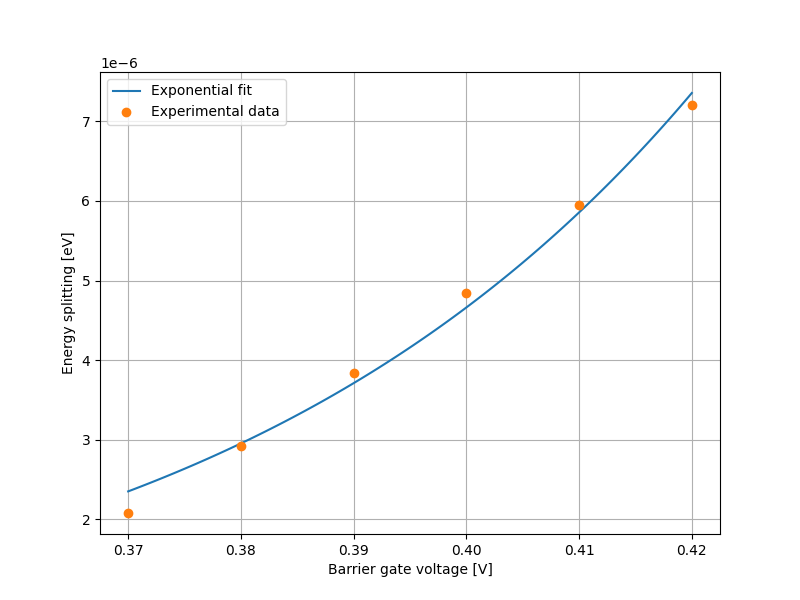
\includegraphics[width=0.7\textwidth]{images/plot.png}
    \caption{Plot of the fitted exponential compared with experimental data}
    \label{plot}
\end{figure}